\section{Analysis}
\label{sec:analysis}

\subsection{Velocity against size}
Figure~\ref{fig:vd} shows the velocity--size relation after each discharge is normalized by its own medians. The per-discharge Theil--Sen slope of $\log v_r$ on $\log \delta_r$ has a median of \vdSlopeMed{} (\vdSlopeMedLo--\vdSlopeMedHi) and is positive in \vdSlopePosShare\% of discharges; the pooled slope is \vdSlopePooled{} (\vdSlopePooledLo--\vdSlopePooledHi) with Spearman $\rho = \vdRhoPooled$. The relation is far from both limiting scalings: the sheath-connected $\delta^{-2}$ is excluded, and the inertial $\delta^{1/2}$ lies well above the interval.

\begin{figure}[t]
\centering
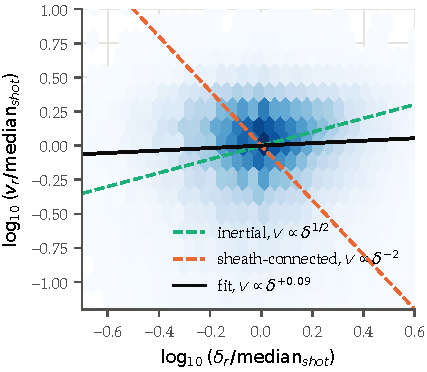
\includegraphics[width=0.55\linewidth]{figs/fig_vd.pdf}
\caption{Radial velocity against radial width, each normalized by the median of its discharge, for all selected tracks (hexagonal bin density). The solid line is the pooled Theil--Sen fit; dashed lines are the sheath-connected and inertial scalings through the medians.}
\label{fig:vd}
\end{figure}

\subsection{Exposure blur}
A filament that moves during the exposure is smeared along its direction of motion, and faster filaments are smeared more, which produces a positive velocity--width correlation with no physical content. The median smear $v_r t_{\rm exp}$ is \blurMedCm{}~cm, about a tenth of the median width, so the effect is small but not negligible. Two tests bound it. First, the slope depends on exposure in the expected direction within M6, where the two common settings share the optics: the per-discharge slope has a median of \vdSlopeExpSeven{} (\vdSlopeExpSevenLo--\vdSlopeExpSevenHi) at 7~$\mu$s ($n = \nExpSeven$) and \vdSlopeExpTen{} (\vdSlopeExpTenLo--\vdSlopeExpTenHi) at 10~$\mu$s ($n = \nExpTen$), while the median width is the same, \dMedExpSeven{} against \dMedExpTen{}~cm, because the extra smear of 3~$\mu$s at 400~m/s is 0.1~cm. The 4~$\mu$s discharges belong to M7 and M8 and are not comparable in width, but their slope, \vdSlopeExpFour{} (\vdSlopeExpFourLo--\vdSlopeExpFourHi), is also low.
Second, correcting each width for its own smear in quadrature lowers the pooled slope to \vdSlopePooledBlur{} (\vdSlopePooledBlurLo--\vdSlopePooledBlurHi). We take this corrected value as the measurement: the radial velocity is nearly independent of width over the measured range, with at most a weak positive dependence.

\begin{figure}[t]
\centering
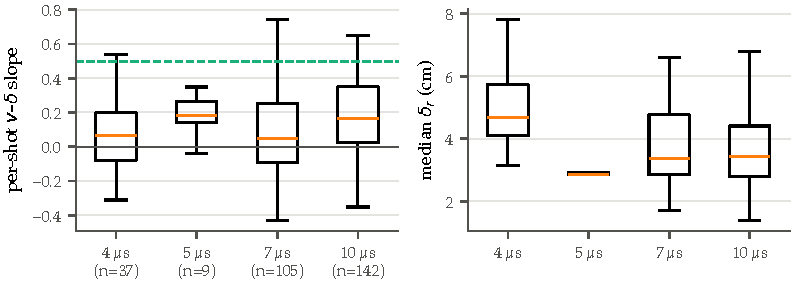
\includegraphics[width=\linewidth]{figs/fig_exposure.pdf}
\caption{Effect of exposure time. Left: per-discharge velocity--width slopes by exposure setting; the dashed line is the inertial scaling. Right: per-discharge median width by exposure.}
\label{fig:exposure}
\end{figure}

\subsection{Two-region normalization}
With the inputs of Section~\ref{sec:method}, the median reference scales are $a^* = \aStarMed$~cm, $v^* = \vStarMed$~m/s, and $\Lambda = \LambdaMed$, so the discharges sit in the low-collisionality half of the regime diagram. Figure~\ref{fig:regimes} places each discharge at its median $\hat a = (\delta_r/2)/a^*$ and $\hat v = v_r/v^*$. The filaments span $\hat a = \aHatMin$--$\aHatMax$ (median \aHatMed), which straddles the velocity maximum of the model; over the central half of this range the model's $\hat v(\hat a)$ stays within a factor of two of its peak. A sample that straddles the peak is expected to show a weak net dependence of velocity on size, and this is what we measure. The normalized velocity, however, is $\hat v \approx \vHatMed$: the measured filaments move at a few percent of the model's velocity scale. Part of this gap is the input assumptions, since $v^* \propto T_e^{7/10}$ and $T_e$ at the LCFS is assumed for \nTeAssumed{} of the \nShotsStats{} discharges, and part is the model itself, which gives the velocity of an isolated, fully formed filament with an order-unity prefactor that simulations in realistic geometry find to be below one \citep{walkden2015characterization, paruta2018blob}. The measurement is also made within 15~cm of the limb, where filaments are still forming and accelerating. The ratio is nonetheless larger than the prefactor uncertainty alone explains, and we regard the amplitude, not the size dependence, as the point of tension with the model.

\begin{figure}[t]
\centering
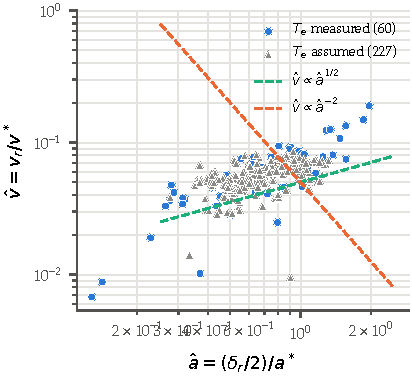
\includegraphics[width=0.55\linewidth]{figs/fig_regimes.pdf}
\caption{Per-discharge median velocity and size in two-region units. Dashed lines are the inertial ($\hat v = \hat a^{1/2}$) and sheath-connected ($\hat v = \hat a^{-2}$) branches. Circles use a measured $T_e$ at the LCFS; triangles assume $T_e = \teDefault$~eV.}
\label{fig:regimes}
\end{figure}

\subsection{Dependence on plasma parameters}
Figure~\ref{fig:params} shows the per-discharge medians against plasma current and Greenwald fraction for the \nShotsL{} non-ELMy discharges, which span $I_p = \ipMin$--\ipMax{}~kA and $f_{\rm GW} = \fgwMin$--\fgwMax. No dependence is resolved. The log--log slope of the median velocity on plasma current is \slVIp{} (\slVIpLo--\slVIpHi) and on Greenwald fraction \slVFgw{} (\slVFgwLo--\slVFgwHi); for the width the slopes are \slDIp{} (\slDIpLo--\slDIpHi) and \slDFgw{} (\slDFgwLo--\slDFgwHi). Beam power has no effect on the velocity (\slVNbi, \slVNbiLo--\slVNbiHi) and a small positive one on the width (\slDNbi, \slDNbiLo--\slDNbiHi). Because these fits pool configurations with different calibrations, we repeat them inside the best-calibrated configuration alone (``\bestCfgView'', \nShotsBestCfgL{} non-ELMy discharges at one scale, $I_p = \ipBestMin$--\ipBestMax{}~kA): the velocity slopes are \slBVIp{} (\slBVIpLo--\slBVIpHi) on current and \slBVFgw{} (\slBVFgwLo--\slBVFgwHi) on Greenwald fraction, consistent with the pooled result.
\citet{kirk2016filaments} found in a dedicated current scan at fixed density and power that the radial velocity falls with current. Our sample is not a controlled scan: current, density, heating, and campaign vary together, and most discharges sit near 700~kA, so a weak dependence is within the reach of confounding. We report the slopes as they are and do not claim a contradiction.

\begin{figure}[t]
\centering
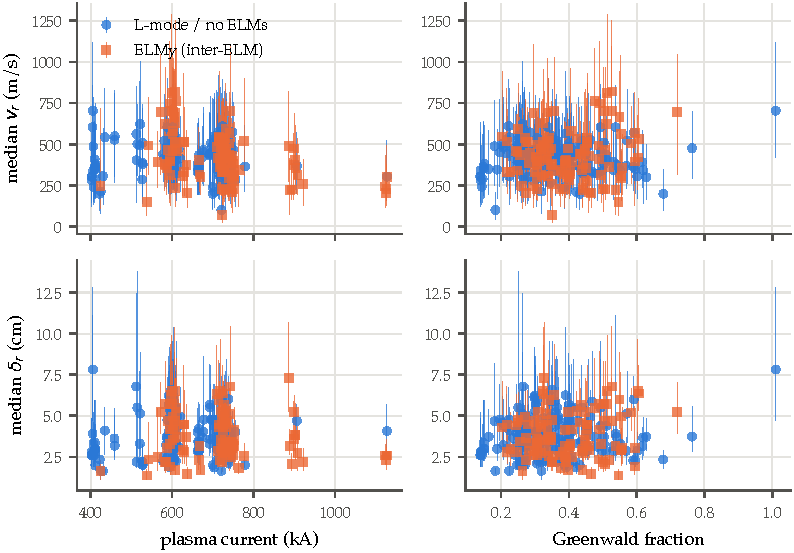
\includegraphics[width=\linewidth]{figs/fig_params.pdf}
\caption{Per-discharge median radial velocity (top) and width (bottom) against plasma current (left) and Greenwald fraction (right). Bars are interquartile ranges over tracks. Circles are discharges without ELMs in the camera window; squares are ELMy discharges, measured between ELMs.}
\label{fig:params}
\end{figure}
